\chapter{Emotion Driven Sentiment Analysis Framework for Edge Devices}
Edge devices can manage the large volumes of unstructured data generated by continuous connectivity. Analyzing this data to understand people's actions has boosted the popularity of emotion detection and sentiment analysis. The most common way people express their feelings is through written text. Emotion recognition can be automated using natural language processing. Recent developments in attention-based approaches and deep learning (DL) have strengthened support for research in this area. \cite{ref55}.

\section{Emotion Recognition}
Comments, posts, and reviews on social media platforms like Instagram, Reddit, Facebook, and Twitter help us infer users' emotional states, such as happiness, appreciation, enthusiasm, pride, rage, fear, anxiety, sadness, and curiosity. Emotion recognition is the detailed analysis of human emotions. Despite the frequent interchangeability of the terms, sentiment analysis and emotion recognition are actually separate concepts \cite{ref28} .

Emotional or psychological states include a broad spectrum of mental conditions, such as joy, enthusiasm, grief, and bewilderment. One application of emotion recognition is the examination of mental health records to identify potential offenders \cite{ref51}, \cite{ref52}. Natural language processing applications that leverage DL require data centers and specialized hardware. However, issues like data isolation, user privacy, and high operational costs hinder NLP development. Because traditional ML algorithms rely on centralized data for training, they face challenges in meeting General Data Protection Rule (GDPR) requirements and building user trust. FL is a decentralized approach that complies with GDPR and enhances data protection and privacy. This emerging method for emotion-driven sentiment analysis in a federated environment helps ensure privacy and improve performance.

\section{Strategic Approach to Framework Development}
Traditional text classification methods rely on high-dimensional, low-density lexical features, such as n-gram representations, and use linear models, such as Support Vector Machines (SVM) or logistic regression. Numerous neural network and transformer techniques, such as LSTM and CNN, have enhanced the proficiency of ML models. But these techniques focus on model performance without considering the size or memory constraints of edge devices. In \cite{ref76}, authors proposed an on-device neural network model for user privacy. They developed self-governing Neural Network (SGNN) and SGNN+ models. These models were static and could classify short text. In \cite{ref75} , the authors developed the Projected Attention Network (PRADO), a trainable projection network to capture long text with an attention mechanism.

In improving emotion guessing via federated learning, PRADO offers a practical approach to achieve better model performance while protecting user privacy. By leveraging PRADO's efficient and reliable on-device neural network design, the method incorporates collaborative weight operations supported by the FL framework. The collaboration enables effective, client-side model aggregation that is both secure and scalable, enabling real-time processing.

\subsection{Proposed PRADO-based emotion recognition}
The projected attention neural network-based federated learning framework is an innovative concept that integrates the simultaneous federated training of projections, attention processes, and convolutions. Figure 3.1 shows the architecture in more detail. The framework is composed of:

\begin{itemize}
    \item Local transformation module: Several client devices execute the text data within each user model with the help of the PRADO system, but do not share the raw data. A local model is trained, and only the learned parameters are uploaded to a central server.
    \item Server module: A federated averaging model is aggregated from local model updates to obtain a global model. The new parameters are then sent to all of the clients for the subsequent training round.
\end{itemize}

The right-hand side displays the PRADO model's internal structure. The long input text is then converted to short, trainable embeddings (as shown in the lower part of Figure 3.1) and passed through several convolution and attention modules.

\begin{figure}[htbp]
  \centering
  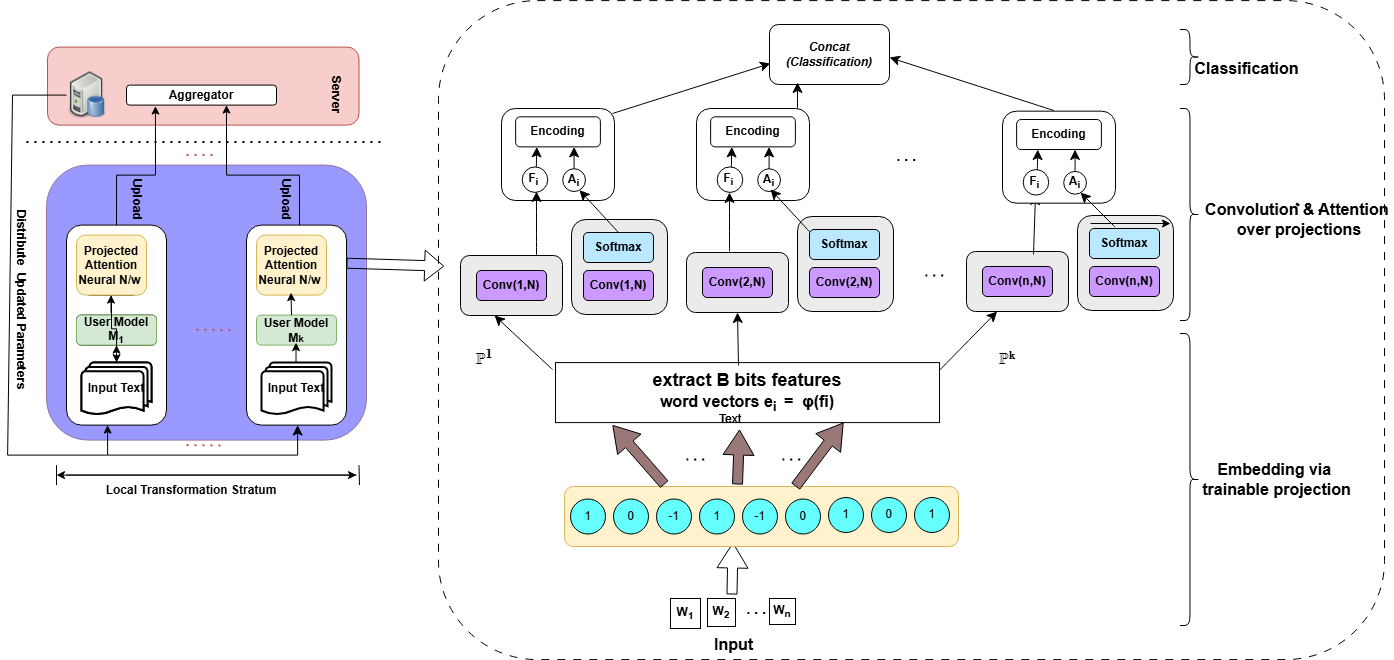
\includegraphics[width=0.8\textwidth]{figures/image15}
  \caption{Federated Learning Framework for Emotion Recognition using PRADO}
  \label{fig:ch3_f1}
\end{figure}

It learns local and contextual semantic properties (middle part of Figure 3.1). The extracted features from various projections are encoded, then combined, and then fed to a classification layer containing a Softmax function for predicting the emotion class (Upper part of Figure 3.1).

\subsection{Working of the PRADO model}
The objective of the PRADO is to classify the emotions using a compact neural network architecture on resource-constrained edge devices. Conventional deep learning models require a large vocabulary and high-dimensional embedding matrices. Using a projection operation, PRADO dynamically generates trainable embeddings. This reduces memory requirements. As discussed earlier, the PRADO model comprises projected embeddings, convolution-based extraction, attention-based feature weighting, and classification. The PRADO process is described using equations (3.2) to (3.8) from \cite{ref75}.

Let an input consist of a sequence of $T$ tokens $\omega_0$, $\omega_1$, $\omega_2$, \ldots, $\omega_{T-1}$. Here $\omega_i$ represents $i$-th token. This token refers to a pre-processed individual word from the input text. The pre-processing may include converting text to lowercase, separating punctuation symbols, and tokenizing the sentence into individual words.

Example: - “I like the rose flowers.” is tokenized as { I, like, the, rose, flowers }. Each token is processed before contextual information is extracted.

In traditional NLP models, each word $\omega_i$ is mapped to a one-hot vector, where $|V|$ is the vocabulary size. It contains a value `1' at the index corresponding to this token and zeros elsewhere. Then, the embedding layer maps to the words,

\begin{equation}
  e_{i} = W \delta_{i}, \quad e_{i} \in \mathbb{R}^{d}
  \label{eq:ch3_3_1}
\end{equation}

\noindent Where $e_{i}$ represents the embedding (or encoded vector) corresponding to the $i$-th token, and it is a $d$-dimensional real-valued vector. $W$ is a weight (or embedding) matrix, typically of size $|V| \times d$, where $|V|$ is the vocabulary size and $d$ is the embedding dimension. $\delta_{i}$ is a one-hot vector of size $|V|$.

This illustration captures semantic information effectively, but the embedding matrix size is proportional to vocabulary size and hence requires large memory storage. This makes the technique unsuitable for edge devices.

\subsubsection{Projected Embedding Layer:}
PRADO addresses this problem by replacing standard embeddings with a projection operation. Each token is transformed into a compact binary fingerprint by applying a hashing function. It generates compact embeddings by hashing each word to a 2B-bit fingerprint. It partitions this into B, 2-bit groups and maps each group to a ternary value in $\{-1, 0, 1\}$. B represents the projection dimension. This results in a projection vector $f_{i}$.

Consider the same example, “I like the rose flowers”. Tokens generated are {I, likes, the, rose, flowers}. Suppose the token “like” is selected. Conventional embedding methods look up the word “like” in a large vocabulary table; instead, PRADO generates a numerical representation via a projection operation.

\subsubsection{Step 1: Generate fingerprint}
The word ''like'' is first run through a hashing function, which produces a binary fingerprint. Suppose that the hash function generates an 8-bit fingerprint.

like $\rightarrow$ 10110010

In practice, PRADO has much longer fingerprints - 256 or 512 bits are common. Here is a short fingerprint (for demonstration purposes only).

\subsubsection{Step 2: Divide the fingerprint into 2-Bit groups}
The binary fingerprint is divided into 2-bit groups. E.g., $10\ 11\ 00\ 10$.

\subsubsection{Step 3: Map each pair to a ternary value}

Each 2-Bit pair in the above sequence is mapped to a ternary value using the following rule: $\{00 \rightarrow 0,\ 01 \rightarrow 1,\ 10 \rightarrow -1,\ 11 \rightarrow 1\}$. Applying this mapping to the word ``like'' 8-bit fingerprint, the projection vector becomes $\{-1,\ 1,\ 0,\ -1\}$.

\subsubsection{Step 4: Trainable projection layer}
The projection vector is transformed into a dense embedding through a trainable linear layer, producing a trainable projection matrix \cite{ref75}.

\begin{equation}
  e_{i} = \phi(f_{i}) \in \mathbb{R}^{d}
  \label{eq:ch3_3_2}
\end{equation}

Suppose this layer produces $e_{i}$, representing the semantic meaning of the word ``like''.

This provides a compact and dynamically generated embedding. Unlike traditional embedding methods, this approach does not require storing a vocabulary table. Instead, word embeddings are generated dynamically. In this approach, two independent convolutional networks are used: a projected feature network F to capture features and a second attention network A to capture the importance of these features.

\subsubsection{Convolution-based feature extraction:}
Emotions are usually captured through a set of words or short phrases, such as “So bad”, “very happy”, “highly disappointed”. Therefore, PRADO applies one-dimensional feature convolution to learn contextual patterns from a sequence of words and extract n-gram-like features.

\begin{equation}
  F_{i}^{n} = \text{Conv}(e_{i}, n, N)
  \label{eq:ch3_3_3}
\end{equation}

Where $n$ is the width of the convolution kernel, $N$ is the number of convolution filters, and $F_{i}^{n}$ denotes the extracted feature vector.

If n=1(unigram), i.e. one word, e.g. “happy”. If n=2(bigram), two consecutive words, e.g., “very happy”. If n=3(trigram), three consecutive words, e.g., “not very happy”. Thus, convolution enables the model to extract meaningful contextual information.

\subsubsection{Attention Mechanism:}
Convolution extracts local contextual features, but not every word may contribute equally to emotion prediction. Consider the sentence, “The car’s look is unimpressive, but the mileage is excellent”.  Words such as ‘car’s’, ‘is’, and ‘the’ do not provide emotional information, whereas ‘unimpressive’ and ' excellent’ are informative. To automatically identify important words, PRADO applies an attention network. The attention score is computed from the word embeddings in the Attention network to assess feature importance.

\begin{equation}
  A_{i}^{n} = W_{a} \cdot F_{i}^{n} + b_{a}
  \label{eq:ch3_3_4}
\end{equation}

\noindent $A_{i}^{n}$ denotes the raw attention score. To capture the relevance of features at various places over the word sequence, we compute SoftMax, which results in a normalized attention weight for every token position.

\begin{equation}
  \alpha_{i}^{n} = \frac{e^{A_{i}^{n}}}{\sum_{i} e^{A_{j}^{n}}}
  \label{eq:ch3_3_5}
\end{equation}

\noindent $\alpha_{i}^{n}$ denotes the normalized attention weight, which emphasizes the emotionally significant words with higher attention weights, whereas irrelevant words receive lower weights.

\subsubsection{Attention -based encoding}
Finally, normalized attention scores $\alpha_{i}^{n}$ are used to compute a weighted representation of the extracted features.

\begin{equation}
  \varepsilon^{n} = \sum_{i} \alpha_{i}^{n} F_{i}^{n}
  \label{eq:ch3_3_6}
\end{equation}

\noindent $\varepsilon^{n}$ denotes fixed-length encoding corresponding to a convolution kernel of size $n$.

For these encoders  n-gram kernels of sizes 1 to n are utilized. Along with this, masked convolution kernels are used to simulate the effect of Skip-grams.

\subsubsection{Applying Skip-grams}
Skip-Grams capture non-consecutive words separated by one or more intermediate tokens.

Consider the example, “The novel was absolutely wonderful”. A bigram produces “novel was”, whereas a skip-1 bigram produces “novel wonderful” that skips the intermediate words. Due to these features, the model captures long-range semantic relationships.

\subsubsection{Classification Layer}
All encoded vectors $\varepsilon^{n}$ from the previous step are assembled into a unified fixed-length embedding:

\begin{equation}
  \text{Encode}(\text{Text}) = \text{concat}(\mathcal{E}^{1}, \mathcal{E}^{2}, \ldots, \mathcal{E}^{n})
  \label{eq:ch3_3_7}
\end{equation}

\noindent These encoded vectors are concatenated along the feature (axis) dimension. If every encoder produces an $N$-dimensional vector, then the concatenated feature vector has $n \times N$ dimension.

Classification output is obtained using a fully connected feed-forward network, denoted by $\psi$, over the fixed-length encoded text $h$.

The output is given by:

\begin{equation}
  \label{eq:ch3_3_8}
  \hat{y} = \text{softmax}(\psi(h))
\end{equation}

The output represents the probability distribution over emotion classes and the emotion label with maximum probability is selected as the final prediction.

\subsubsection{Aggregation at Server Module}
As demonstrated in Figure 3.1, the predicted probabilities from Local devices are transmitted to the server. The server aggregates all user embeddings from different locations. The buffered FedAvg is applied for the aggregation process that aggregates the received parameters using

\begin{equation}
  u_{r} = f_{\text{agg}}(u_{1}, u_{2}, \ldots, u_{k}; \theta_{A})
  \label{eq:ch3_3_9}
\end{equation}

Where $u_{r}$ are the unified parameters, $f_{\text{agg}}$ is the function that performs federated averaging, and $\theta_{A}$ denotes the parameters of the aggregator model.

The general structure of the Projected Attention Network (PRADO), including projection, convolution, attention, and classification layers, was presented in this section. It also explained how to aggregate model weights from many client devices in the federated learning approach. All of these make for a complete picture of the proposed FL-PRADO framework. In Section 3.3, the practical aspects of the proposed framework are described, along with the experimental setup, data preparation, and dataset details.

\section{Experimental Setup and Dataset}
All experiments in this research were executed end-to-end on an Apple M4 Max workstation (128 GB unified memory), using a GPU via TensorFlow Metal 1.1.0, Python 3.11 with TensorFlow 2.15.1/Keras 2, and scikit-learn 1.9. Every notebook executes top-to-bottom under papermill on the seq-flow-lite-metal kernel. The aggregation server (ML Server; Spring Boot/Kotlin) runs on http://localhost:8080.

\subsubsection*{Dataset Slitting for implementation purposes}
The GoEmotions corpus (43,410 training and 5,427 test examples, 27 emotions + neutral, multi-label) \cite{ref77} is partitioned into 120 client shards of \textasciitilde{}362 examples using a seeded permutation that is persisted to disk, so every training and upload session operates on identical shards. Metrics are reported on the shared test set at the 0.5 decision threshold; precision (P) and recall (R) are micro-averaged, F1 = 2PR/(P+R). The federated server is the MLServer application (Kotlin / Spring Boot); every federated result in this section was produced through a real client-server round trip, not a simulation.

\subsubsection*{Dataset Details}
It only takes a few words for a human to express a wide range of nuanced emotions. A human-annotated dataset of 58,000 Reddit comments, named GoEmotions \cite{ref77}, was produced by Google researchers. This dataset was compiled from various English-language subreddits. Moreover, these feelings are classified into 27 distinct types. Google researchers developed this dataset with consideration for the psychology and usefulness of nuanced emotions in data. A neural network based on the FedL was trained on this dataset to predict emotions. The association between ratings and the hierarchical classification of 27 emotions is shown in Figure 3.2. The positive, negative, and ambiguous sentiments were predetermined. As shown in Figure 3.2, clusters closely match sentiment groupings. As a stand-in for emotional categories, emoji embeddings improve the dataset. Multilingual corpora benefit from this approach.\cite{ref77}. By exploring how the GoEmotions dataset is used to predict emotions, researchers can leverage its extensive range of emotional categories to understand better and classify complex emotional states. Being very selective in terms of filters and offensive material makes it a good starting point to coming up with algorithms that can predict emotions. By using advanced emotion prediction models, including PRADO, researchers can enhance the accuracy and utility of this technique because it excels at text classification and model size optimization. The advantage of these models is the semantic richness of the data in the GoEmotions dataset. The dataset's hierarchical emotion taxonomy also allows us to analyze nuanced emotional variations in detail, giving us better insight into how people feel and how emotion prediction models can be more accurate.  \cite{ref77}.

Using SOTA modeling methodologies, including PRADO, in conjunction with the GoEmotions data would allow us to develop experimental systems that are both effective in prediction accuracy and rich in data. It could be very important for improving emotion prediction.

The limitations of the dataset are  1. According to the GoEmotions dataset, there is an unequal distribution of the categories of emotions. Certain classes of emotions, such as nervousness, pride, and grief, have fewer than 1,000 samples, whereas others, such as admiration, approval, and thanks, have between 10,000 and 12,000 examples. This disparity influences model training and assessment.

The dataset was formed by the English Reddit community and annotated by Indian English speakers. This is biased and doesn't reflect global diversity.

\begin{figure}[htbp]
  \centering
  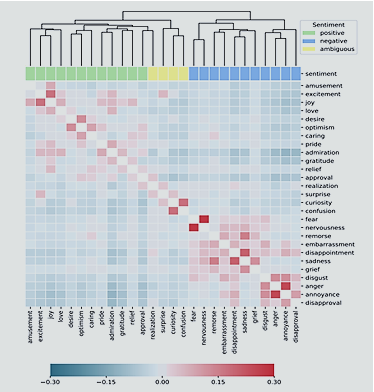
\includegraphics[width=0.55\textwidth]{figures/image16}
  \caption{Correlation and Hierarchical clustering of emotions and their rating \cite{ref77}}
  \label{fig:ch3_f2}
\end{figure}

\section{Results and Discussion}
For evaluating emotion prediction models, the metrics are Precision, Recall, and F1 Score. Although the GoEmotions dataset labeled Reddit comments with 27 emotions, we considered only 12 emotions that are strongly identified.

\subsubsection*{Performance Analysis}
We compare the final results of BERT, Plain PRADO, and FL-PRADO, implemented using the environment discussed in Section 3.3. As per the setup mentioned in Section 3.3, the federated configuration of FL-PRADO includes 120 clients. The GoEmotions dataset is divided into 43,410 training examples and 5,427 test examples over 28 emotions. The BERT and PRADO models are using the dataset as per the train and test split mentioned here. On the other hand, this dataset is divided across 120 clients with approximately 360-365 examples each (seeded permutation, persisted) for FL-PRADO. Precision and Recall were chosen, along with F1 score, due to the nature of emotion recognition being a multi-class classification problem, where a class imbalance can be misleading. These are complementary indicators of how well the model is able to correctly recognize emotions, capture the true emotion instances, and to balance both. For the GoEmotions-based FL-PRADO experiment, Macro-F1 can be especially valuable because it gives each emotion class equal importance, including less frequent emotions.

\subsection{Precision Comparison}
Precision of a model is stated as the proportion of its positive predictions that turn out to be true.

\begin{equation}
  \text{Precision} = \frac{TP}{TP + FP}
  \label{eq:ch3_precision}
\end{equation}

\noindent Where $TP$ is the number of true positives and $FP$ is the number of false positives.

Recall measures the proportion of correct positive predictions out of all actual positives in the data.

\begin{equation}
  \text{Recall} = \frac{TP}{TP + FN}
  \label{eq:ch3_recall}
\end{equation}

\noindent Where $FN$ is the number of false negatives.

The F1-score provides a balanced assessment, considering both Precision and Recall.

\begin{equation}
  \text{F1 Score} = \frac{2 \times \text{Precision} \times \text{Recall}}{\text{Precision} + \text{Recall}}
  \label{eq:ch3_f1}
\end{equation}

\begin{table}[htbp]
  \centering
  \caption{Precision scores for the prediction of emotions}
  \label{tab:ch3_t1}
  \begin{tabular}{|c|c|c|c|}
    \hline
    Emotion & Precision (Small BERT) & Precision PRADO & Precision  FL-PRADO \\
    \hline
    Desire & 0.600 & 0.553 & 0.529 \\
    \hline
    Excitement & 0.667 & 0.710 & 0.278 \\
    \hline
    Amusement & 0.724 & 0.725 & 0.724 \\
    \hline
    Anger & 0.561 & 0.602 & 0.522 \\
    \hline
    Admiration & 0.702 & 0.602 & 0.431 \\
    \hline
    Gratitude & 0.932 & 0.950 & 0.966 \\
    \hline
    Remorse & 0.545 & 0.527 & 0.500 \\
    \hline
    Joy & 0.482 & 0.551 & 0.536 \\
    \hline
    Sadness & 0.562 & 0.594 & 0.461 \\
    \hline
    Love & 0.767 & 0.782 & 0.536 \\
    \hline
    Optimism & 0.713 & 0.713 & 0.680 \\
    \hline
    Neutral & 0.645 & 0.612 & 0.467 \\
    \hline
  \end{tabular}
\end{table}

Table 3.1 displays the precision scores for predicting emotions using three different model setups: Baseline 1 (BERT), Baseline 2 (the original PRADO model); and the PRADO model used in an FL context(FL-PRADO .

\begin{figure}[htbp]
  \centering
  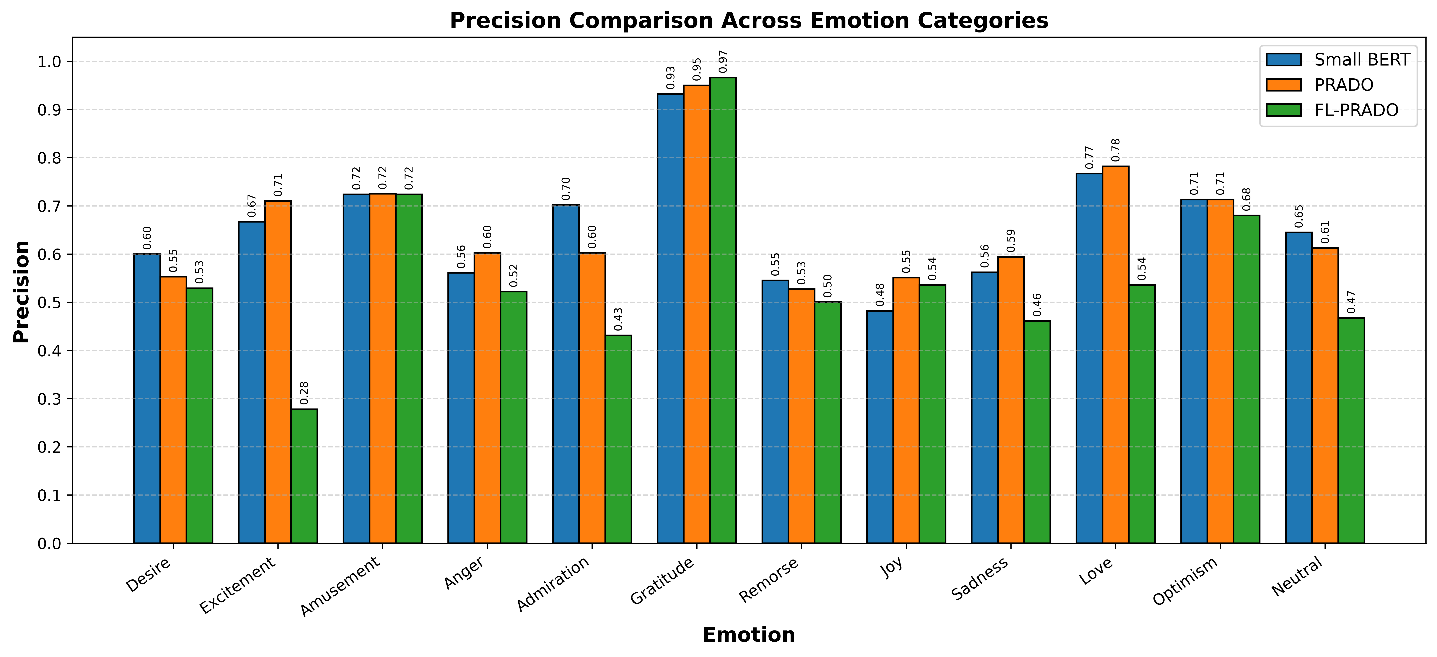
\includegraphics[width=0.8\textwidth]{figures/image17}
  \caption{Precision comparison with base models}
  \label{fig:ch3_f3}
\end{figure}

The bar chart compares the precision scores for predicting emotions using three different model setups: Baseline 1 (BERT), Baseline 2 (with PRADO only), and PRADO used in a Federated Learning (FL) environment. It examines twelve emotions, from admiration to sadness, to assess how well the models can predict whether someone is feeling good. The green bars representing FL-PRADO maintain competitive precision across several emotions while preserving privacy in an FL environment, consistently achieving better precision scores for most emotions. However, the macro-average precision for 27 emotions is lower than that of baseline models.

\subsection{Recall Comparison}
Recall measures the proportion of correct positive predictions out of all actual positives in the data.

As discussed in the dataset limitations, certain emotions have fewer examples than others. Training and Evaluation of the models are affected by this.

Table 3.3 and the bar chart in Figure 3.4 compare recall values for three model configurations across twelve emotional categories. This comparison differs from the earlier precision-focused figure. It shows that FL-PRADO consistently has the highest recall for most emotions.

\begin{table}[htbp]
  \centering
  \caption{Recall@5 score evaluation for emotion prediction}
  \label{tab:ch3_t2}
  \begin{tabular}{|c|c|c|c|}
    \hline
    Emotion & Recall (BERT)- & Recall (PRADO) & Recall (FL-PRADO) \\
    \hline
    Admiration & 0.444 & 0.489 & 0.574 \\
    \hline
    Joy & 0.168 & 0.503 & 0.566 \\
    \hline
    Anger & 0.162 & 0.288 & 0.292 \\
    \hline
    Desire & 0.145 & 0.313 & 0.317 \\
    \hline
    Excitement & 0.117 & 0.214 & 0.149 \\
    \hline
    Gratitude & 0.821 & 0.858 & 0.898 \\
    \hline
    Optimism & 0.306 & 0.468 & 0.476 \\
    \hline
    Love & 0.622 & 0.786 & 0.788 \\
    \hline
    Neutral & 0.558 & 0517 & 0.618 \\
    \hline
    Remorse & 0.321 & 0.696 & 0.589 \\
    \hline
    Sadness & 0.231 & 0.263 & 0.263 \\
    \hline
    Amusement & 0.526 & 0.658 & 0.665 \\
    \hline
  \end{tabular}
\end{table}

Figure 3.4 shows a comparison of Recall for all 3 models mentioned across twelve emotions.  FL PRADO has much better recall values. For example, the recall for admiration (0.574), gratitude (0.898), and joy (566) indicates stricter classification boundaries.

\begin{figure}[htbp]
  \centering
  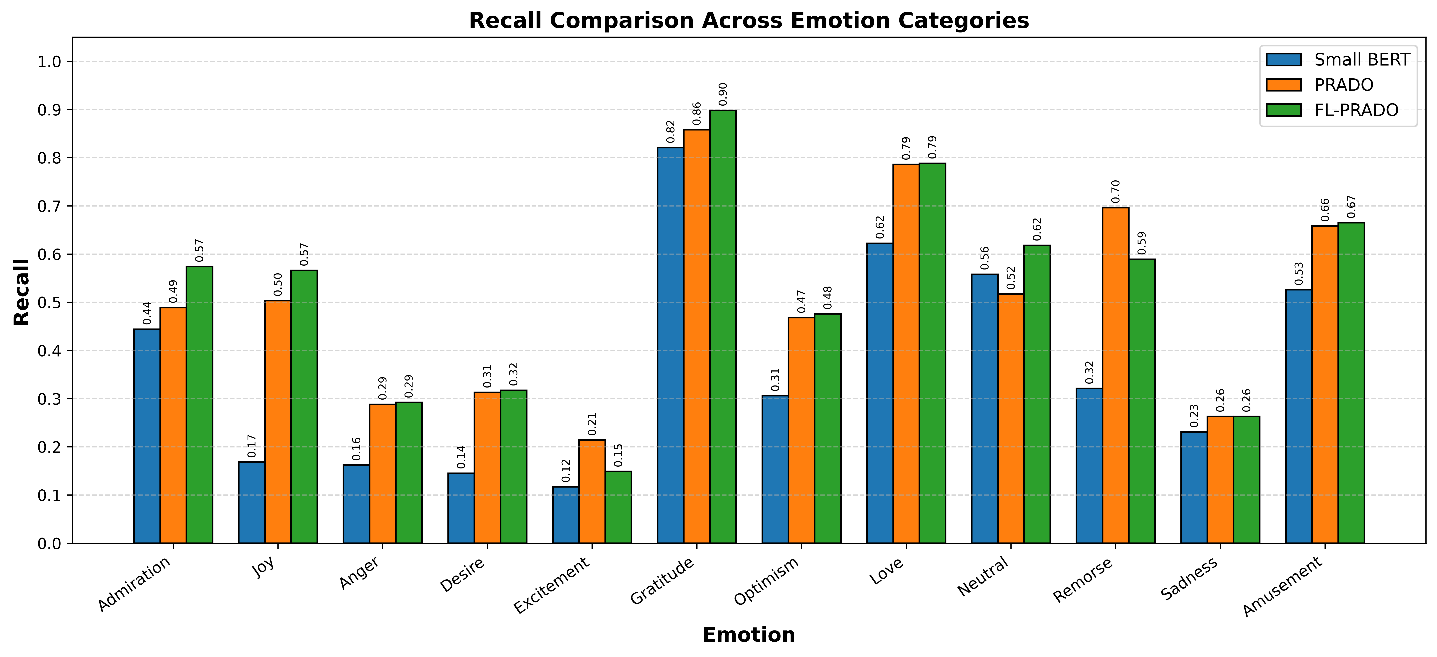
\includegraphics[width=0.8\textwidth]{figures/image18}
  \caption{Recall comparison with base models}
  \label{fig:ch3_f4}
\end{figure}

This higher recall can be beneficial in personalized emotion-based recommendation systems, where offering unrelated emotional content may harm user experience more than omitting a few items. In federated settings, stronger local model behavior also helps protect privacy and reduces noise during aggregation, leading to more accurate and personalized results. Therefore, FL PRADO produces highly reliable predictions, which is crucial for emotion models used in privacy-sensitive applications.

\subsection{F1 Score Comparison}
The F1-score provides a balanced assessment. It considers both Precision and Recall. It is formulated as shown.

The F1 score comparison graph in Figure 3.5 and Table 3.4 shows how well emotion prediction models perform across three different settings: Baseline 1 (BERT), Baseline 2 (PRADO), and FL-PRADO. Baseline 1 has a better F1 score for some emotions. Baseline 2 shows that PRADO has a positive effect on prediction quality in a federation-free system. The PRADO-FL system remains competitive across key emotions such as gratitude, love, and neutrality, demonstrating PRADO's flexibility amid federation constraints. An emotion such as excitement would probably not work, as the data is limited and different for local FL training.

\begin{table}[htbp]
  \centering
  \caption{F1-Score Comparison with Base Models}
  \label{tab:ch3_t3}
  \begin{tabular}{|c|c|c|c|}
    \hline
    Emotion & F1 Score (BERT) & F1 Score (PRADO) & F1 Score (FL-PRADO) \\
    \hline
    Admiration & 0.544 & 0.596 & 0.452 \\
    \hline
    Gratitude & 0.873 & 0.901 & 0.886 \\
    \hline
    Anger & 0.251 & 0.369 & 0.351 \\
    \hline
    Desire & 0.233 & 0.4 & 0.308 \\
    \hline
    Excitement & 0.198 & 0.328 & 0.083 \\
    \hline
    Amusement & 0.610 & 0.596 & 0.452 \\
    \hline
    Joy & 0.249 & 0.523 & 0.435 \\
    \hline
    Love & 0.687 & 0.784 & 0.784 \\
    \hline
    Neutral & 0.598 & 0.561 & 0.588 \\
    \hline
    Optimism & 0.429 & 0.565 & 0.484 \\
    \hline
    Remorse & 0.404 & 0.6 & 0.569 \\
    \hline
    Sadness & 0.327 & 0.364 & 0.355 \\
    \hline
  \end{tabular}
\end{table}

\begin{figure}[htbp]
  \centering
  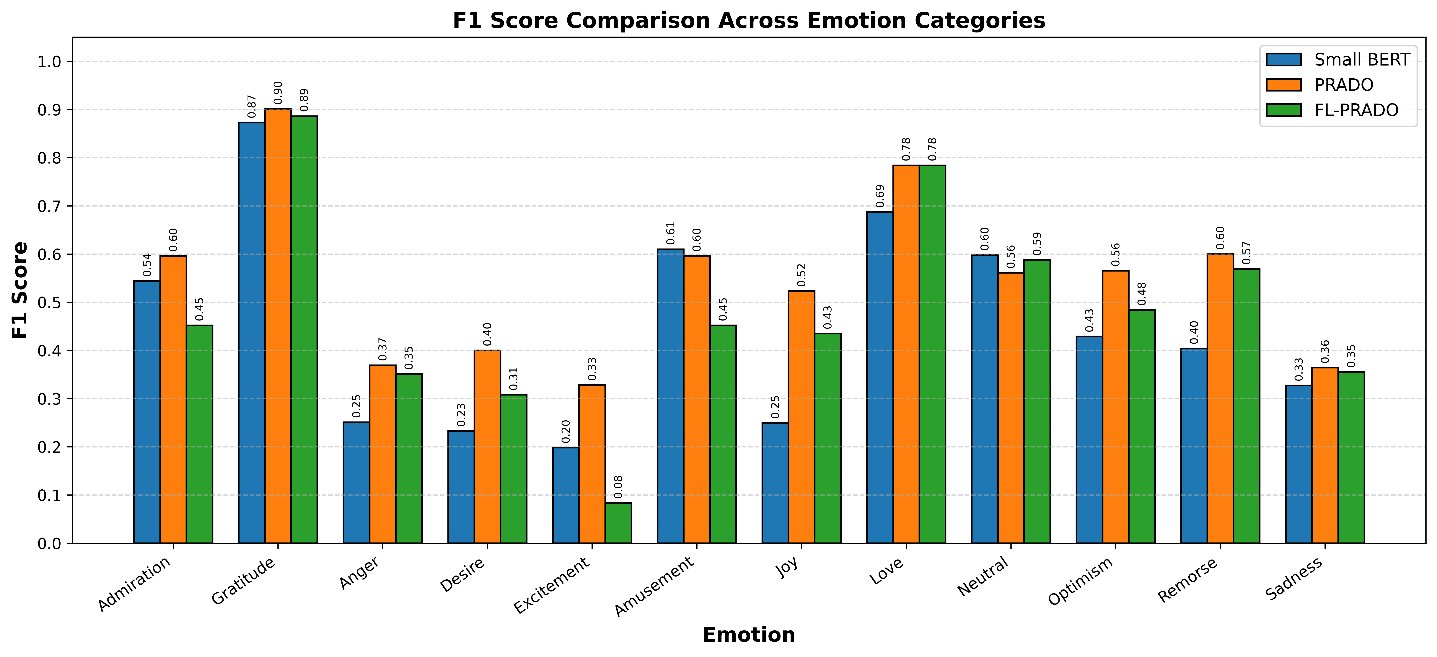
\includegraphics[width=0.8\textwidth]{figures/image19}
  \caption{F1 Score Comparison with Base Models}
  \label{fig:ch3_f5}
\end{figure}

\subsection{Evaluation of Emotion Prediction}
We first run the baseline models---LSTM \cite{ref84}, Bi-LSTM \cite{ref85} , BERT\cite{ref67} , and PRADO---in a non-federated learning (FL) setting. For on-device applications, PRADO's strength is its ability to function well with low memory and processing power. The estimated precision, recall, and F1-score values for various language models are displayed in Table 5.1.

\begin{table}[htbp]
  \centering
  \caption{Emotion prediction analysis using the GoEmotions dataset}
  \label{tab:ch3_t4}
  \begin{tabular}{|c|c|c|c|c|c|}
    \hline
    Model & Setting & Test loss (BCE) & Precision@0.5 & Recall@0.5 & F1-score \\
    \hline
    BERT & centralized & --- & 0.679 & 0.351 & 0.463 \\
    \hline
    PRADO & (on device) & 0.327 & 0.630 & 0.392 & 0.483 \\
    \hline
    LSTM & centralized & --- & 0.642 & 0.351 & 0.453 \\
    \hline
    Bi-LSTM & centralized & --- & 0.673 & 0.292 & 0.407 \\
    \hline
    BERT FL & federated & 0.138 & 0.596 & 0.256 & 0.358 \\
    \hline
    PRADO FL & federated & 0.174 & 0.467 & 0.476 & 0.472 \\
    \hline
  \end{tabular}
\end{table}

Every baseline model---LSTM, Bi-LSTM, BERT, and PRADO---is executed in a typical, non-FL setting. Compared to other models, FL-PRADO exhibits notable advancements in Recall and F1 score. We computed the 95\% confidence intervals (CI) for accuracy, recall, and F1-score to give a statistical measure of their dependability and variability. The models were re-evaluated on random subsets of the test set at ten sizes (10\%, 20\%, $\ldots$ 100\%), and their 95\% confidence intervals were obtained by bootstrapping $B = 1{,}000$ resamples within that subset.  Various clients and training cycles are represented by weighted-average scores of various variables in Tables 3.5(a)--3.5(c) and Figures 3.6(a)--3.6(c).

\setlength{\tabcolsep}{4pt}
\begin{longtable}{|p{1.9cm}|p{1.9cm}|p{1.9cm}|p{1.9cm}|p{1.9cm}|p{1.9cm}|p{1.9cm}|}
\caption{Weighted-averaged Precision: realized value on each evaluation subset}
\label{tab:ch3_t5} \\
\hline
Eval. size & BERT & PRADO & LSTM & Bi-LSTM & BERT FL & PRADO FL \\
\hline
\endfirsthead
\hline
Eval. size & BERT & PRADO & LSTM & Bi-LSTM & BERT FL & PRADO FL \\
\hline
\endhead
\hline
\endfoot
10\% / (n=543) & 0.645 / {[0.568, 0.706]} & 0.562 / {[0.479, 0.613]} & 0.527 / {[0.450, 0.589]} & 0.284 / {[0.244, 0.329]} & 0.324 / {[0.247, 0.373]} & 0.394 / {[0.356, 0.447]} \\
\hline
20\% / (n=1,085) & 0.621 / {[0.559, 0.661]} & 0.537 / {[0.482, 0.587]} & 0.573 / {[0.522, 0.620]} & 0.385 / {[0.332, 0.419]} & 0.355 / {[0.320, 0.391]} & 0.438 / {[0.407, 0.474]} \\
\hline
30\% / (n=1,628) & 0.669 / {[0.631, 0.707]} & 0.549 / {[0.514, 0.596]} & 0.583 / {[0.527, 0.631]} & 0.357 / {[0.310, 0.382]} & 0.379 / {[0.320, 0.407]} & 0.437 / {[0.410, 0.462]} \\
\hline
40\% / (n=2,171) & 0.676 / {[0.619, 0.709]} & 0.522 / {[0.499, 0.551]} & 0.596 / {[0.536, 0.621]} & 0.332 / {[0.310, 0.356]} & 0.377 / {[0.324, 0.399]} & 0.456 / {[0.422, 0.482]} \\
\hline
50\% / (n=2,714) & 0.615 / {[0.579, 0.654]} & 0.552 / {[0.518, 0.595]} & 0.598 / {[0.549, 0.625]} & 0.359 / {[0.313, 0.378]} & 0.379 / {[0.331, 0.400]} & 0.434 / {[0.410, 0.452]} \\
\hline
60\% / (n=3,256) & 0.667 / {[0.618, 0.695]} & 0.534 / {[0.515, 0.557]} & 0.591 / {[0.539, 0.614]} & 0.365 / {[0.323, 0.383]} & 0.382 / {[0.333, 0.402]} & 0.463 / {[0.425, 0.482]} \\
\hline
70\% / (n=3,799) & 0.657 / {[0.630, 0.687]} & 0.553 / {[0.521, 0.589]} & 0.590 / {[0.547, 0.612]} & 0.364 / {[0.323, 0.380]} & 0.379 / {[0.334, 0.397]} & 0.452 / {[0.424, 0.474]} \\
\hline
80\% / (n=4,342) & 0.656 / {[0.622, 0.687]} & 0.540 / {[0.515, 0.574]} & 0.582 / {[0.546, 0.607]} & 0.367 / {[0.330, 0.384]} & 0.389 / {[0.344, 0.406]} & 0.446 / {[0.425, 0.469]} \\
\hline
90\% / (n=4,884) & 0.657 / {[0.625, 0.687]} & 0.558 / {[0.528, 0.592]} & 0.596 / {[0.558, 0.618]} & 0.372 / {[0.330, 0.387]} & 0.385 / {[0.341, 0.400]} & 0.446 / {[0.425, 0.468]} \\
\hline
100\% / (n=5,427) & 0.656 / {[0.627, 0.684]} & 0.549 / {[0.520, 0.582]} & 0.592 / {[0.555, 0.614]} & 0.365 / {[0.328, 0.378]} & 0.380 / {[0.336, 0.396]} & 0.457 / {[0.430, 0.475]} \\
\hline
\end{longtable}

The weighted-averaged precision with 95\% confidence intervals (CI) for BERT, LSTM, Bi-LSTM, PRADO, and FL-PRADO across different dataset sizes is shown in Fig.  3.2(a). Compared to FL models, BERT, PRADO, and Bi-LSTM demonstrate higher precision. As the evaluation set size increases, the confidence intervals narrow. FL-PRADO achieves the best recall results for all evaluation-set sizes. The model's high recall across all iterations indicates greater sensitivity to the positive emotion classes in the federated learning framework, which helps maintain predictive capacity while minimizing missed detections. The 95\% half-width of the weighted F1 is reduced from around $\pm 0.035$--$0.041$ at 10\% of the test set to $\pm 0.012$--$0.013$ at the full test set. The interval width doesn't shrink monotonically over all models, due to the different random subset of evaluations used by each evaluation size.

\begin{figure}[htbp]
  \centering
  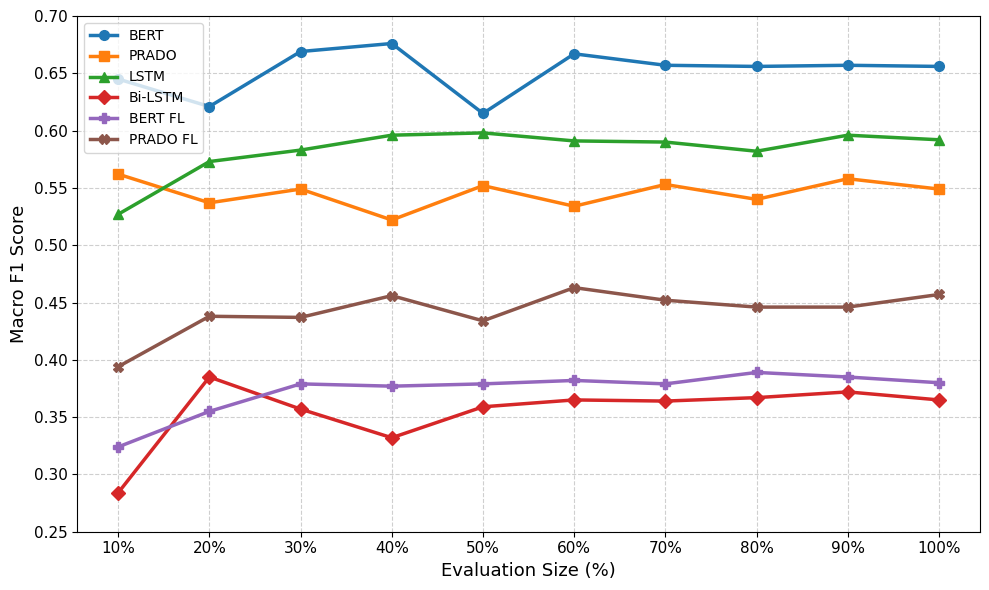
\includegraphics[width=\textwidth]{figures/image20}
  \caption{Weighted-averaged precision with 95\% CI for different models}
  \label{fig:ch3_f6}
\end{figure}

\begin{longtable}{|p{1.9cm}|p{1.9cm}|p{1.9cm}|p{1.9cm}|p{1.9cm}|p{1.9cm}|p{1.9cm}|}
\caption{Weighted-averaged Recall: realized value on each evaluation subset}
\label{tab:ch3_t6} \\
\hline
Eval. Size & BERT & PRADO & LSTM & Bi-LSTM & BERT FL & PRADO FL \\
\hline
\endfirsthead
\hline
Eval. Size & BERT & PRADO & LSTM & Bi-LSTM & BERT FL & PRADO FL \\
\hline
\endhead
\hline
\endfoot
10\% / (n=543) & 0.350 / {[0.313, 0.385]} & 0.387 / {[0.348, 0.428]} & 0.352 / {[0.318, 0.388]} & 0.269 / {[0.236, 0.302]} & 0.234 / {[0.200, 0.268]} & 0.460 / {[0.422, 0.500]} \\
\hline
20\% / (n=1,085) & 0.341 / {[0.317, 0.369]} & 0.398 / {[0.372, 0.425]} & 0.380 / {[0.353, 0.407]} & 0.311 / {[0.286, 0.337]} & 0.262 / {[0.238, 0.288]} & 0.498 / {[0.468, 0.526]} \\
\hline
30\% / (n=1,628) & 0.349 / {[0.329, 0.370]} & 0.395 / {[0.375, 0.420]} & 0.346 / {[0.324, 0.370]} & 0.280 / {[0.261, 0.301]} & 0.246 / {[0.228, 0.269]} & 0.471 / {[0.449, 0.494]} \\
\hline
40\% / (n=2,171) & 0.349 / {[0.331, 0.369]} & 0.392 / {[0.371, 0.409]} & 0.346 / {[0.326, 0.363]} & 0.283 / {[0.264, 0.301]} & 0.254 / {[0.237, 0.273]} & 0.473 / {[0.454, 0.493]} \\
\hline
50\% / (n=2,714) & 0.349 / {[0.333, 0.367]} & 0.390 / {[0.374, 0.408]} & 0.349 / {[0.332, 0.365]} & 0.290 / {[0.274, 0.306]} & 0.250 / {[0.234, 0.265]} & 0.466 / {[0.448, 0.483]} \\
\hline
60\% / (n=3,256) & 0.361 / {[0.345, 0.376]} & 0.401 / {[0.387, 0.417]} & 0.352 / {[0.338, 0.367]} & 0.293 / {[0.279, 0.308]} & 0.259 / {[0.246, 0.274]} & 0.481 / {[0.464, 0.497]} \\
\hline
70\% / (n=3,799) & 0.354 / {[0.340, 0.370]} & 0.390 / {[0.376, 0.404]} & 0.353 / {[0.339, 0.368]} & 0.294 / {[0.281, 0.308]} & 0.259 / {[0.245, 0.273]} & 0.474 / {[0.459, 0.489]} \\
\hline
80\% / (n=4,342) & 0.353 / {[0.337, 0.366]} & 0.392 / {[0.378, 0.405]} & 0.353 / {[0.340, 0.365]} & 0.292 / {[0.280, 0.305]} & 0.260 / {[0.247, 0.271]} & 0.480 / {[0.467, 0.494]} \\
\hline
90\% / (n=4,884) & 0.354 / {[0.341, 0.367]} & 0.396 / {[0.384, 0.410]} & 0.353 / {[0.341, 0.365]} & 0.296 / {[0.284, 0.308]} & 0.257 / {[0.245, 0.269]} & 0.480 / {[0.468, 0.494]} \\
\hline
100\% / (n=5,427) & 0.351 / {[0.340, 0.364]} & 0.392 / {[0.381, 0.404]} & 0.351 / {[0.339, 0.362]} & 0.292 / {[0.280, 0.304]} & 0.256 / {[0.245, 0.266]} & 0.476 / {[0.464, 0.489]} \\
\hline
\end{longtable}

\begin{figure}[htbp]
  \centering
  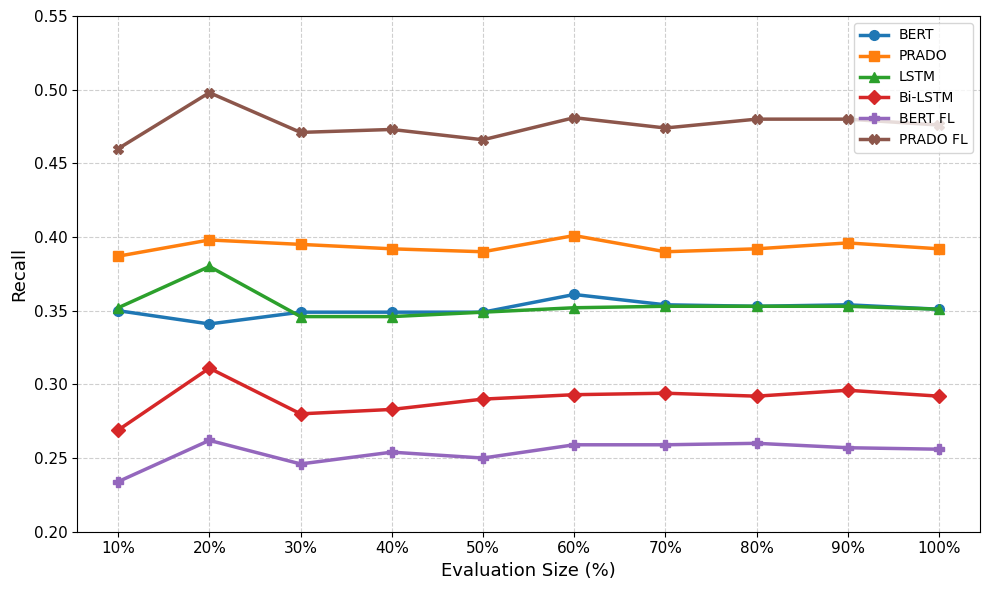
\includegraphics[width=\textwidth]{figures/image21}
  \caption{Weighted-averaged Recall with 95\% confidence intervals}
  \label{fig:ch3_f7}
\end{figure}

\begin{longtable}{|p{1.9cm}|p{1.9cm}|p{1.9cm}|p{1.9cm}|p{1.9cm}|p{1.9cm}|p{1.9cm}|}
\caption{Weighted-averaged F1: realized value on each evaluation subset}
\label{tab:ch3_t7} \\
\hline
Eval. size & BERT & PRADO & LSTM & Bi-LSTM & BERT FL & PRADO FL \\
\hline
\endfirsthead
\hline
Eval. size & BERT & PRADO & LSTM & Bi-LSTM & BERT FL & PRADO FL \\
\hline
\endhead
\hline
\endfoot
10\% / (n=543) & 0.408 / {[0.365, 0.443]} & 0.420 / {[0.379, 0.462]} & 0.385 / {[0.344, 0.424]} & 0.275 / {[0.240, 0.311]} & 0.237 / {[0.203, 0.272]} & 0.387 / {[0.348, 0.427]} \\
\hline
20\% / (n=1,085) & 0.400 / {[0.371, 0.430]} & 0.433 / {[0.404, 0.460]} & 0.423 / {[0.392, 0.451]} & 0.331 / {[0.304, 0.359]} & 0.265 / {[0.237, 0.293]} & 0.426 / {[0.397, 0.454]} \\
\hline
30\% / (n=1,628) & 0.418 / {[0.394, 0.441]} & 0.434 / {[0.413, 0.458]} & 0.393 / {[0.367, 0.416]} & 0.301 / {[0.279, 0.323]} & 0.260 / {[0.239, 0.284]} & 0.407 / {[0.385, 0.430]} \\
\hline
40\% / (n=2,171) & 0.406 / {[0.385, 0.426]} & 0.427 / {[0.407, 0.446]} & 0.392 / {[0.369, 0.411]} & 0.303 / {[0.284, 0.322]} & 0.260 / {[0.242, 0.280]} & 0.410 / {[0.390, 0.431]} \\
\hline
50\% / (n=2,714) & 0.407 / {[0.388, 0.427]} & 0.430 / {[0.413, 0.448]} & 0.392 / {[0.374, 0.409]} & 0.306 / {[0.289, 0.323]} & 0.261 / {[0.244, 0.277]} & 0.402 / {[0.385, 0.419]} \\
\hline
60\% / (n=3,256) & 0.423 / {[0.405, 0.439]} & 0.439 / {[0.423, 0.455]} & 0.398 / {[0.380, 0.414]} & 0.312 / {[0.296, 0.328]} & 0.269 / {[0.255, 0.285]} & 0.417 / {[0.400, 0.433]} \\
\hline
70\% / (n=3,799) & 0.417 / {[0.401, 0.433]} & 0.430 / {[0.414, 0.446]} & 0.397 / {[0.382, 0.413]} & 0.312 / {[0.297, 0.327]} & 0.268 / {[0.254, 0.283]} & 0.409 / {[0.394, 0.423]} \\
\hline
80\% / (n=4,342) & 0.414 / {[0.399, 0.429]} & 0.433 / {[0.418, 0.446]} & 0.399 / {[0.384, 0.413]} & 0.312 / {[0.298, 0.326]} & 0.271 / {[0.258, 0.284]} & 0.415 / {[0.401, 0.429]} \\
\hline
90\% / (n=4,884) & 0.417 / {[0.404, 0.431]} & 0.437 / {[0.423, 0.451]} & 0.400 / {[0.385, 0.412]} & 0.316 / {[0.303, 0.329]} & 0.270 / {[0.258, 0.283]} & 0.415 / {[0.402, 0.429]} \\
\hline
100\% / (n=5,427) & 0.413 / {[0.400, 0.426]} & 0.433 / {[0.419, 0.444]} & 0.396 / {[0.383, 0.408]} & 0.311 / {[0.298, 0.323]} & 0.267 / {[0.255, 0.279]} & 0.411 / {[0.398, 0.423]} \\
\hline
\end{longtable}
\setlength{\tabcolsep}{6pt}

\begin{figure}[htbp]
  \centering
  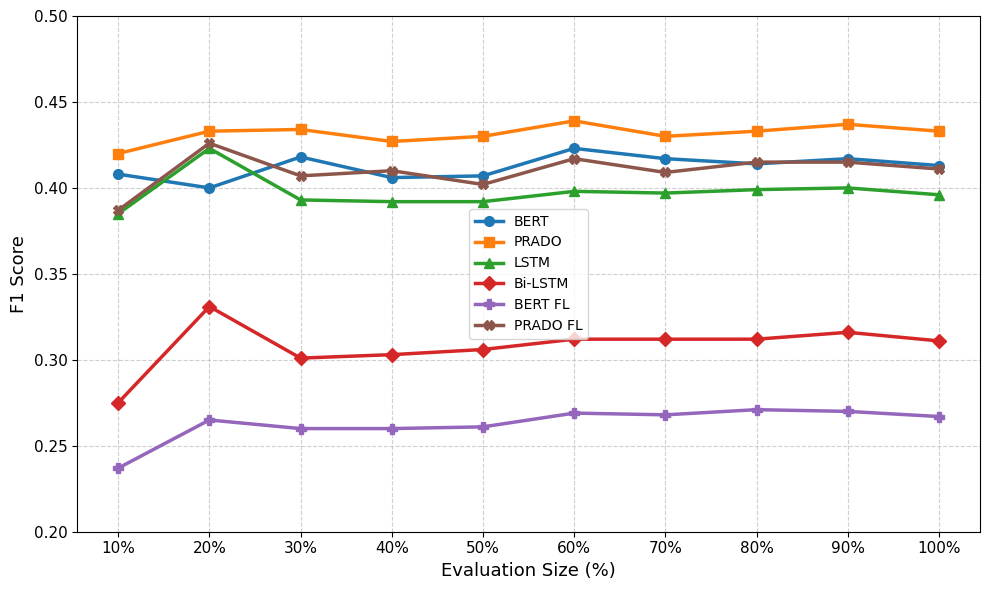
\includegraphics[width=\textwidth]{figures/image22}
  \caption{Weighted-averaged F1 score with 95\% confidence intervals}
  \label{fig:ch3_f8}
\end{figure}

\section{Detailed Analysis of Work}
This section provides details regarding the selection of models for comparison and the performance of the proposed model for research. The purpose of this experimentation is to check the suitability of PRADO in the FL framework.

\subsection{Model Selection for 12 strongly identified emotions Comparison}
The proposed work compares FL-PRADO, BERT, and PRADO. All three models are trained on the GoEmotions dataset using the setup given in Section 3.3. The BERT model is a representative pre-trained transformer model and is also used by the authors of PRADO for comparison. Considering the challenges of FL environment, \cite{ref28} and the lightweight projection-based architecture of PRADO, we integrated it into the FL framework. To assess the performance of the proposed model only for emotion prediction, the models required should be common in the dataset used for training. Hence, BERT is selected as a representative transformer model, and PRADO is selected as it is ideal for its lightweight framework. The proposed model can be compared with other SOTA models for emotion prediction, but these models are either using centralized machine learning without considering user privacy or FL models that use different datasets and provide no publicly available implementation details to reproduce them. To create a common platform for further research work, these three models were implemented and assessed across Precision, Recall, and F1.

\subsection{Performance discussion of proposed model}
The objective of FL-PRADO is not only to enhance evaluation metrics, but also to address three practical requirements: First, privacy preservation by ensuring that the user’s original data never leaves the local device. Second, lightweight deployment using PRADO is most suitable for edge devices participating in federated learning. Third, the work carried out in this chapter demonstrated scalable collaborative learning across 120 distributed clients.

Considering these requirements, the performance of FL-PRADO is justifiable. The precision analysis over several emotions produces competitive performance (desire, amusement, anger, gratitude, etc.), though the macro average is poor. FL-PRADO achieves the highest recall for most emotions, and the performance of FL-PRADO is very close to the performance of PRADO for F1-Score.

\section{Summary}
In this chapter, we proposed a framework for privacy-preserving emotion recognition, called FL-PRADO. It included a detailed description of the PRADO architecture, the federation aggregation process, the experimental setup, dataset partitioning, and the GoEmotions dataset. The effectiveness of the proposed model was tested in terms of Precision, recall, and F1 score. The results were compared with baseline models. The results show that FL-PRADO can make competitive emotion prediction without compromising user privacy and enables efficient deployment on edge devices. These emotion predictions are used in the following chapter to create the proposed cross-domain recommendation framework. The work described in this chapter demonstrates the accomplishment of the first and second objectives. According to a research survey, no federated learning framework has been implemented using PRADO for emotion prediction.

